\documentclass[11  pt]{article} 
\usepackage[lmargin=1in,rmargin=1.75in,bmargin=1in,tmargin=1in]{geometry}  

\input{preamble}
\usepackage{graphicx}
\usepackage{amsmath}
\usepackage{amssymb}


\begin{document}
\onehalfspacing

\lecture{2: Fast Fourier Transforms}{August 27, 2026}

\paragraph{Course Logistics}

\begin{itemize}
\item Read Chapter 30 of the textbook for today's material on the FFT.
\item Syllabus quiz, HW, intro video due Fri, Sep 4.
\end{itemize}

\section{Motivation: Polynomial Multiplication}

We will introduce a powerful application of the divide and conquer paradigm: the Fast Fourier Transform (FFT). We will motivate it through the problem of polynomial multiplication.

\begin{definition} \noindent A \hide{\textbf{polynomial}} in the variable $x$ over an algebraic field is a representation of a function $A(x)$ as a formal sum:
    \begin{equation*}
        A(x) = \sum_{j=0}^{n-1} a_j x^j
    \end{equation*}
    The values $a_0, a_1, \hdots, a_{n-1}$ are the \hide{\textbf{coefficients}} of the polynomial. 
\end{definition}

\vs{.5cm}

\begin{example}\textbf{Polynomial Multiplication} \\
\framebox{
\vbox{
\textbf{Input}: Two polynomials $A(x) = \sum_{j=0}^{n-1} a_j x^j$ and $B(x) = \sum_{j=0}^{n-1} b_j x^j$ of degree bound $n$.
    
\textbf{Output:} A polynomial $C(x) = A(x)B(x)$ of degree bound $2n-1$ such that:
    \begin{equation*}
    C(x) = \sum_{j=0}^{2n-2} c_j x^j \quad \text{where} \quad c_j = \sum_{k=0}^{j} a_k b_{j-k}
    \end{equation*}
}}

\vs{5pt}

An instance of this problem is multiplying $A(x) = 2 + x + 3x^2 + x^3$ and $B(x) = 1 + 2x + 4x^2 + x^3$.
\end{example}

\newpage
Compute $C(x)=A(x)\cdot B(x)$, where $A(x) = 2 + x + 3x^2 + x^3$ and $B(x) = 1 + 2x + 4x^2 + x^3$.

\vs{3in}

Notice that each coefficient $c_j=\sum_{k=0}^j a_kb_{j-k}$ is formed by multiplying pairs of coefficients whose indices sum to $j$, and adding the resulting products together. This operation is called a \hide{convolution}.

\vs{0.5in}

\QU What is the asymptotic runtime of multiplying two polynomials of degree bound $n$ using the standard, na\"{i}ve approach?
\begin{enumerate}
    \aitem $O(1)$
    \bitem $O(n)$
    \citem $O(n \log n)$
    \ditem $O(n^2)$
    \eitem Other
\end{enumerate}
\end{Qu}
%D

\vs{1in}

Compute $C(1)$ for $C(x)=A(x)\cdot B(x)$, where $A(x) = 2 + x + 3x^2 + x^3$ and $B(x) = 1 + 2x + 4x^2 + x^3$.

%$$x^6 + 7x^5 + 15x^4 + 13x^3 + 13x^2 + 5x + 2$$

\newpage
\section{Representations of Polynomials}
To multiply polynomials faster, we can change how we represent them.

\subsection{Coefficient Representation}
We represent $A(x)$ as a vector of coefficients $a = (a_0, a_1, \hdots, a_{n-1})$.
\begin{itemize}
    \item Evaluating $A(x)$ at a given point takes \hide{$O(n)$} time.
    \item Multiplying two polynomials takes \hide{$O(n^2)$} time.
\end{itemize}

\subsection{Point-Value Representation}
A polynomial of degree bound $n$ is uniquely determined by its values at $n$ distinct points. 
We can represent $A(x)$ as a set of $n$ point-value pairs:
\begin{equation*}
    \{ (x_0, y_0), (x_1, y_1), \hdots, (x_{n-1}, y_{n-1}) \}
\end{equation*}
where $y_k = A(x_k)$ for $k = 0, 1, \hdots, n-1$.

\vs{0.5cm}

\textbf{Why use point-value representation?} \\
If we have $A$ and $B$ in point-value form evaluated at the \emph{same} points $x_0, \hdots, x_{2n-1}$, how long does it take to compute $C(x) = A(x)B(x)$ in point-value form? \\

Since \hide{$C(x_k) = A(x_k)B(x_k)$}, we just multiply the $y$-values! This takes \hide{$O(n)$} time!

\vs{1in}

Compute $C(1)$ for $C(x)=A(x)\cdot B(x)$, where $A(x) = 2 + x + 3x^2 + x^3$ and $B(x) = 1 + 2x + 4x^2 + x^3$, by computing and multiplying $A(1)$ and $B(1)$. 

\vs{2in}

\QU Which of the following is the smallest number of point-value pairs that suffices to compute the polynomial $C(x) = A(x)B(x)$ uniquely, assuming $A$ and $B$ have degree bound $n$?
\begin{enumerate}
    \aitem $n$
    \bitem $2n$
    \citem $n\log n$
    \ditem $n^2$
\end{enumerate}
\end{Qu}

\vs{0.5cm}
\paragraph{The Strategy:}
\begin{itemize}
    \item \textbf{Evaluate}: Convert $A$ and $B$ to point-value form at $2n$ points.
    \item \textbf{Point-wise Multiply}: Multiply all pairs of values in \hide{$O(n)$} total time.
    \item \textbf{Interpolate}: Convert $C$ back to coefficient form.
\end{itemize}

Suppose we evaluate $A(x) = 2 + x + 3x^2 + x^3$ at $x=1,2,3,\ldots,10$. 

\begin{equation*}
\begin{bmatrix}
        A(1) \\ A(2) \\ A(3) \\ \vdots \\ A(10)
    \end{bmatrix}
		=
    \begin{bmatrix}
        y_1 \\ y_2 \\ y_3 \\ \vdots \\ y_{10}
    \end{bmatrix}
    =
    \begin{bmatrix}
        1 & 1 & 1 & 1 \\
        1 & 2 & 4 & 8 \\
        1 & 3 & 9 & 27 \\
        \vdots & \vdots & \vdots & \vdots \\
        1 & 10 & 100 & 1000
    \end{bmatrix}
    \begin{bmatrix}
        2 \\ 1 \\ 3 \\ 1
    \end{bmatrix}
\end{equation*}

More generally, if we evaluate $A(x) = \sum_{j=0}^{n-1} a_j x^j$ at points $x_1,\ldots,x_n$, we are computing:

\begin{equation*}
    \begin{bmatrix}
        y_1 \\ y_2 \\ y_3 \\ \vdots \\ y_n
    \end{bmatrix}
    =
    \begin{bmatrix}
        1 & x_1 & x_1^2 & \cdots & x_1^{n-1} \\
				1 & x_2 & x_2^2 & \cdots & x_2^{n-1} \\
				1 & x_3 & x_3^2 & \cdots & x_3^{n-1} \\
        \vdots & \vdots & \vdots & \ddots & \vdots \\
        1 & x_n & x_n^2 & \cdots & x_n^{n-1} \\
    \end{bmatrix}
    \begin{bmatrix}
        a_0 \\ a_1 \\ a_2 \\ \vdots \\ a_{n-1}
    \end{bmatrix}
\end{equation*}

\vs{1cm}
\noindent
If we use arbitrary points, Evaluation and Interpolation take \hide{$O(n^2)$} time in total. We need to choose our evaluation points strategically!

\newpage
\section{The Divide-and-Conquer Strategy}
We have seen that representing a polynomial by its values at $n$ points makes multiplication easy, but converting between coefficient and point-value representations naively takes \hide{$O(n^2)$} time.

\vs{1cm}

Our goal is therefore to speed up polynomial evaluation using \hide{divide-and-conquer}.

\vs{1cm}

Consider
\[A(x) = \sum_{j=0}^{n-1} a_j x^j.\]

\vs{2cm}

Observe that we can separate the even and odd powers:
\begin{align*}
A(x)
&= \sum_j a_{2j}x^{2j} + \sum_j a_{2j+1}x^{2j+1} \\
&= \sum_j a_{2j}(x^2)^j
   + x\sum_j a_{2j+1}(x^2)^j.
\end{align*}

\vs{2cm}

Define the two polynomials
\[
A_{\mathrm{even}}(z) = \sum_j a_{2j}z^j,
\qquad
A_{\mathrm{odd}}(z) = \sum_j a_{2j+1}z^j.
\]

\vs{2cm}

Then

\vs{1cm}

\[\hide{
\boxed{
A(x) = A_{\mathrm{even}}(x^2)
      + xA_{\mathrm{odd}}(x^2).
}}
\]

%\vs{0.5cm}
\newpage
This suggests a divide-and-conquer strategy. Suppose we want to
evaluate $A$ at $n$ points
\[
x_0,x_1,\ldots,x_{n-1}.
\]
If the squared points
\[
x_0^2,x_1^2,\ldots,x_{n-1}^2
\]
contain only $n/2$ distinct values, then we only need to evaluate
$A_{\mathrm{even}}$ and $A_{\mathrm{odd}}$ at $n/2$ points each.

Thus, evaluating $A$ at $n$ points reduces to:
\begin{itemize}
    \item evaluating $A_{\mathrm{even}}$ at $n/2$ points;
    \item evaluating $A_{\mathrm{odd}}$ at $n/2$ points;
    \item combining the resulting values in $O(n)$ time.
\end{itemize}

This gives the recurrence
\[\hide{T(n) = 2T(n/2) + O(n),}\]
which solves to
\[\hide{T(n) = O(n\log n).}\]

\vs{0.5cm}

So the key question is:

\begin{center}
\emph{Can we find $n$ distinct evaluation points whose squares contain only $n/2$ distinct values?}
\end{center}

The answer will lead us to the \textbf{complex roots of unity}.

\newpage
\section{Background Math: Complex Roots of Unity}
Our current goal is to find $n$ distinct values whose squares contain only $n/2$ distinct values. 

\vs{1cm}

Let's see if we can find such a set of numbers by solving the equation $x^n = 1$ over the complex numbers. Let's try small powers of 2:

\vs{1cm}

\begin{itemize}
    \item $n=1: x^1 = 1 \implies x = $ \hide{$1$}
    \item $n=2: x^2 = 1 \implies x = $ \hide{$1, -1$}
    \item $n=4: x^4 = 1 \implies x = $ \hide{$1, -1, i, -i$}
    \item $n=8: x^8 = 1 \implies x = $ \hide{$\pm 1, \pm i, \pm \frac{\sqrt{2}}{2} \pm i\frac{\sqrt{2}}{2}$}
\end{itemize}

\vs{1cm}

Notice an incredible pattern! The solutions for $n=4$ contain the solutions for $n=2$. Crucially, if we take our set of four solutions to $x^4=1$ and \emph{square} them all, we get $\{1, 1, -1, -1\}$, which is exactly the set of two distinct solutions to $x^2=1$. 

\vs{1cm}

\textbf{Algorithmic Takeaway:} Squaring these points halves the number of distinct values! This is exactly the property we need to split our problem size in half for a divide-and-conquer algorithm.

\vs{1cm}

\begin{definition} \noindent The \textbf{$n$-th complex roots of unity} are the $n$ complex numbers $\omega$ such that:
    \begin{equation*}
        \hide{\omega^n = 1}
    \end{equation*}
    They are given by the formula:
    \begin{equation*}
        \omega_n^k = e^{2\pi i k / n} \quad \text{for } k = 0, 1, \hdots, n-1
    \end{equation*}
\end{definition}

\newpage
\paragraph{The Unit Circle.}
In the complex plane, the \hide{\textbf{unit circle}} is the set of complex numbers whose distance from the origin is $1$. 

\vs{1cm}

The \hide{complex roots of unity} all lie on the unit circle, and form a regular polygon inscribed inside the unit circle.

\begin{figure}[h]
    \centering
    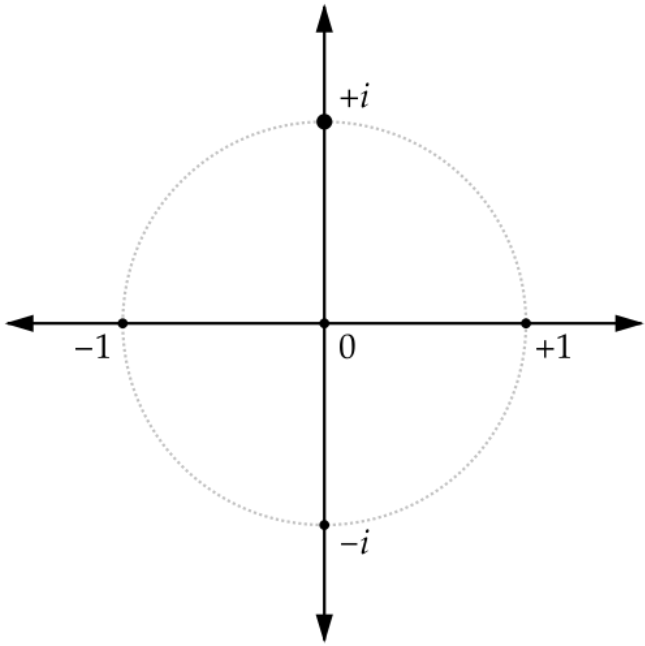
\includegraphics[width=0.4\textwidth]{roots.png}
    \caption{The complex roots of unity equally spaced around the unit circle.}
\end{figure}

To represent these points, we use \textbf{Euler's Formula}:
\begin{equation*}
    e^{i\theta} = \cos(\theta) + i\sin(\theta)
\end{equation*}

\vs{1cm}

Furthermore, \textbf{De Moivre's Theorem} (which follows from standard exponent rules) states that exponentiating a complex number simply multiplies its angle: 
\begin{equation*}
    (e^{i\theta})^m = e^{im\theta} = \cos(m\theta) + i\sin(m\theta)
\end{equation*}

\vs{0.5cm}

This implies that taking powers of our roots of unity does not blow up to huge numbers; it simply \emph{rotates} the value around the unit circle!

\vs{0.5cm}

This formula gives us the coordinates of a point on the unit circle at angle $\theta$. 
Since a full circle is $2\pi$ radians, we can generate all $n$ distinct $n$-th roots of unity by taking evenly spaced angles: $\theta = 2\pi k / n$.


\begin{lemma}\textbf{Summation Lemma:} For any integer $n \geq 1$ and non-zero integer $k$ not divisible by $n$:
    \begin{equation*}
        \sum_{j=0}^{n-1} (\omega_n^k)^j = \hide{0}
    \end{equation*}
\end{lemma}

\newpage

\section{Intuition for the Fast Fourier Transform}

Recall $A(x) = A_{\mathrm{even}}(x^2) + xA_{\mathrm{odd}}(x^2)$ needs to be evaluated at $n$ different values of $x$. 
Suppose we evaluate $A_{\mathrm{even}}(x^2)$ at 
%\[x=\hide{1,\omega,\omega^2,\omega^3,\ldots,\omega^{n-1}},\]

\vs{1in}

where $\omega$ is an $n$-th root of unity and $n$ is a power of $2$. 
Then 
%\[x^2=\hide{1,\omega^2,\omega^4,\ldots,\omega^{n-2}},\]

\vs{2in}

All we need to do is evaluate $A_{\mathrm{even}}(x^2)$ at $\frac{n}{2}$ points!

\vs{0.3in}

To recover $A(x) = A_{\mathrm{even}}(x^2) + xA_{\mathrm{odd}}(x^2)$ at $x=1,\omega,\omega^2,\omega^3,\ldots,\omega^{n-1}$, also need to evaluate $A_{\mathrm{odd}}(x^2)$ at $\frac{n}{2}$ points. 
Here is the pseudocode for the recursive FFT algorithm, which evaluates a polynomial at the $n$-th roots of unity.

\begin{algorithm}
    \caption{Recursive-FFT($a$)}
    \begin{algorithmic}
        \State $n = \textbf{length}(a)$
        \If{$n == 1$}
        \State Return $a$
        \EndIf
        \State $\omega_n = e^{2\pi i / n}$
        \State $\omega = 1$
        \State $a^{[0]} = (a_0, a_2, \hdots, a_{n-2})$
        \State $a^{[1]} = (a_1, a_3, \hdots, a_{n-1})$
        \State $y^{[0]} = \textsc{Recursive-FFT}(a^{[0]})$
        \State $y^{[1]} = \textsc{Recursive-FFT}(a^{[1]})$
        \State Let $y$ be a new array of length $n$
        \For{$k = 0$ to $n/2 - 1$}
            \State $y_k = y^{[0]}_k + \omega \cdot y^{[1]}_k$
            \State $y_{k + n/2} = y^{[0]}_k - \omega \cdot y^{[1]}_k$
            \State $\omega = \omega \cdot \omega_n$
        \EndFor
        \State Return $y$
    \end{algorithmic}
\end{algorithm}


\newpage
\section{The Matrix Perspective (Discrete Fourier Transform)}
Consider an example for $n=8$, so $\omega$ is an eighth-root of unity, $\omega^8=1$. 
\begin{equation*}
    \begin{bmatrix}
        y_0 \\ y_1 \\ y_2 \\ y_3 \\ y_4 \\ y_5 \\ y_6 \\ y_7
    \end{bmatrix}
    =
    \begin{bmatrix}
        1 & 1 & 1 & 1 & 1 & 1 & 1 & 1 \\
        1 & \omega & \omega^2 & \omega^3 & \omega^4 & \omega^5 & \omega^6 & \omega^7 \\
        1 & \omega^2 & \omega^4 & \omega^6 & \omega^8 & \omega^{10} & \omega^{12} & \omega^{14} \\
        1 & \omega^3 & \omega^6 & \omega^9 & \omega^{12} & \omega^{15} & \omega^{18} & \omega^{21} \\
        1 & \omega^4 & \omega^8 & \omega^{12} & \omega^{16} & \omega^{20} & \omega^{24} & \omega^{28} \\
        1 & \omega^5 & \omega^{10} & \omega^{15} & \omega^{20} & \omega^{25} & \omega^{30} & \omega^{35} \\
        1 & \omega^6 & \omega^{12} & \omega^{18} & \omega^{24} & \omega^{30} & \omega^{36} & \omega^{42} \\
        1 & \omega^7 & \omega^{14} & \omega^{21} & \omega^{28} & \omega^{35} & \omega^{42} & \omega^{49}
    \end{bmatrix}
    \begin{bmatrix}
        a_0 \\ a_1 \\ a_2 \\ a_3 \\ a_4 \\ a_5 \\ a_6 \\ a_7
    \end{bmatrix}.
\end{equation*}

\vs{1in}

\begin{equation*}
    \begin{bmatrix}
        y_0 \\ y_1 \\ y_2 \\ y_3 \\ y_4 \\ y_5 \\ y_6 \\ y_7
    \end{bmatrix}
    =
    \begin{bmatrix}
        \omega^0 & \omega^0 & \omega^0 & \omega^0 & \omega^0 & \omega^0 & \omega^0 & \omega^0 \\
        \omega^0 & \omega & \omega^2 & \omega^3 & \omega^4 & \omega^5 & \omega^6 & \omega^7 \\
        \omega^0 & \omega^2 & \omega^4 & \omega^6 & \omega^0 & \omega^2 & \omega^4 & \omega^6 \\
        \omega^0 & \omega^3 & \omega^6 & \omega & \omega^4 & \omega^7 & \omega^2 & \omega^5 \\
        \omega^0 & \omega^4 & \omega^0 & \omega^4 & \omega^0 & \omega^4 & \omega^0 & \omega^4 \\
        \omega^0 & \omega^5 & \omega^2 & \omega^7 & \omega^4 & \omega & \omega^6 & \omega^3 \\
        \omega^0 & \omega^6 & \omega^4 & \omega^2 & \omega^0 & \omega^6 & \omega^4 & \omega^2 \\
        \omega^0 & \omega^7 & \omega^6 & \omega^5 & \omega^4 & \omega^3 & \omega^2 & \omega
    \end{bmatrix}
    \begin{bmatrix}
        a_0 \\ a_1 \\ a_2 \\ a_3 \\ a_4 \\ a_5 \\ a_6 \\ a_7
    \end{bmatrix}.
\end{equation*}

\vs{1in}

\begin{equation*}
    \begin{bmatrix}
        y_0 \\ y_1 \\ y_2 \\ y_3 \\ y_4 \\ y_5 \\ y_6 \\ y_7
    \end{bmatrix}
    =
    \begin{bmatrix}
        \color{blue}{\omega^0} & \color{red}{\omega^0} & \color{blue}{\omega^0} & \color{red}{\omega^0} & \color{blue}{\omega^0} & \color{red}{\omega^0} & \color{blue}{\omega^0} & \color{red}{\omega^0} \\
        \color{blue}{\omega^0} & \color{red}{\omega^1} & \color{blue}{\omega^2} & \color{red}{\omega^3} & \color{blue}{\omega^4} & \color{red}{\omega^5} & \color{blue}{\omega^6} & \color{red}{\omega^7} \\
        \color{blue}{\omega^0} & \color{red}{\omega^2} & \color{blue}{\omega^4} & \color{red}{\omega^6} & \color{blue}{\omega^0} & \color{red}{\omega^2} & \color{blue}{\omega^4} & \color{red}{\omega^6} \\
        \color{blue}{\omega^0} & \color{red}{\omega^3} & \color{blue}{\omega^6} & \color{red}{\omega^1} & \color{blue}{\omega^4} & \color{red}{\omega^7} & \color{blue}{\omega^2} & \color{red}{\omega^5} \\
        \color{blue}{\omega^0} & \color{red}{\omega^4} & \color{blue}{\omega^0} & \color{red}{\omega^4} & \color{blue}{\omega^0} & \color{red}{\omega^4} & \color{blue}{\omega^0} & \color{red}{\omega^4} \\
        \color{blue}{\omega^0} & \color{red}{\omega^5} & \color{blue}{\omega^2} & \color{red}{\omega^7} & \color{blue}{\omega^4} & \color{red}{\omega^1} & \color{blue}{\omega^6} & \color{red}{\omega^3} \\
        \color{blue}{\omega^0} & \color{red}{\omega^6} & \color{blue}{\omega^4} & \color{red}{\omega^2} & \color{blue}{\omega^0} & \color{red}{\omega^6} & \color{blue}{\omega^4} & \color{red}{\omega^2} \\
        \color{blue}{\omega^0} & \color{red}{\omega^7} & \color{blue}{\omega^6} & \color{red}{\omega^5} & \color{blue}{\omega^4} & \color{red}{\omega^3} & \color{blue}{\omega^2} & \color{red}{\omega^1}
    \end{bmatrix}
    \begin{bmatrix}
        \color{blue}{a_0} \\ \color{red}{a_1} \\ \color{blue}{a_2} \\ \color{red}{a_3} \\ \color{blue}{a_4} \\ \color{red}{a_5} \\\color{blue}{a_6} \\ \color{red}{a_7}
    \end{bmatrix}.
\end{equation*}

\vs{1in}

\begin{equation*}
    \begin{bmatrix}
        y_0 \\ y_2 \\ y_4 \\ y_6 \\ y_1 \\ y_3 \\ y_5 \\ y_7
    \end{bmatrix}
    =
    \begin{bmatrix}
        \color{blue}{\omega^0} & \color{blue}{\omega^0} & \color{blue}{\omega^0} & \color{blue}{\omega^0} &
        \color{red}{\omega^0} & \color{red}{\omega^0} & \color{red}{\omega^0} & \color{red}{\omega^0} \\
        \color{blue}{\omega^0} & \color{blue}{\omega^2} & \color{blue}{\omega^4} & \color{blue}{\omega^6} &
        \color{red}{\omega^1} & \color{red}{\omega^3} & \color{red}{\omega^5} & \color{red}{\omega^7} \\
        \color{blue}{\omega^0} & \color{blue}{\omega^4} & \color{blue}{\omega^0} & \color{blue}{\omega^4} &
        \color{red}{\omega^2} & \color{red}{\omega^6} & \color{red}{\omega^2} & \color{red}{\omega^6} \\
        \color{blue}{\omega^0} & \color{blue}{\omega^6} & \color{blue}{\omega^4} & \color{blue}{\omega^2} &
        \color{red}{\omega^3} & \color{red}{\omega^1} & \color{red}{\omega^7} & \color{red}{\omega^5} \\
        \color{blue}{\omega^0} & \color{blue}{\omega^0} & \color{blue}{\omega^0} & \color{blue}{\omega^0} &
        \color{red}{\omega^4} & \color{red}{\omega^4} & \color{red}{\omega^4} & \color{red}{\omega^4} \\
        \color{blue}{\omega^0} & \color{blue}{\omega^2} & \color{blue}{\omega^4} & \color{blue}{\omega^6} &
        \color{red}{\omega^5} & \color{red}{\omega^7} & \color{red}{\omega^1} & \color{red}{\omega^3} \\
        \color{blue}{\omega^0} & \color{blue}{\omega^4} & \color{blue}{\omega^0} & \color{blue}{\omega^4} &
        \color{red}{\omega^6} & \color{red}{\omega^2} & \color{red}{\omega^6} & \color{red}{\omega^2} \\
        \color{blue}{\omega^0} & \color{blue}{\omega^6} & \color{blue}{\omega^4} & \color{blue}{\omega^2} &
        \color{red}{\omega^7} & \color{red}{\omega^5} & \color{red}{\omega^3} & \color{red}{\omega^1}
    \end{bmatrix}
    \begin{bmatrix}
        \color{blue}{a_0} \\ \color{blue}{a_2} \\ \color{blue}{a_4} \\ \color{blue}{a_6} \\ \color{red}{a_1} \\ \color{red}{a_3} \\ \color{red}{a_5} \\ \color{red}{a_7}
    \end{bmatrix}.
\end{equation*}

Four matrix multiplications:

\begin{equation*}
\begin{bmatrix}
    \color{blue}{\omega^0} & \color{blue}{\omega^0} & \color{blue}{\omega^0} & \color{blue}{\omega^0} \\
    \color{blue}{\omega^0} & \color{blue}{\omega^2} & \color{blue}{\omega^4} & \color{blue}{\omega^6} \\
    \color{blue}{\omega^0} & \color{blue}{\omega^4} & \color{blue}{\omega^0} & \color{blue}{\omega^4} \\
    \color{blue}{\omega^0} & \color{blue}{\omega^6} & \color{blue}{\omega^4} & \color{blue}{\omega^2}
\end{bmatrix}
\begin{bmatrix}
        \color{blue}{a_0} \\ \color{blue}{a_2} \\ \color{blue}{a_4} \\ \color{blue}{a_6}
    \end{bmatrix}
\qquad
\begin{bmatrix}
    \color{red}{\omega^0} & \color{red}{\omega^0} & \color{red}{\omega^0} & \color{red}{\omega^0} \\
    \color{red}{\omega^1} & \color{red}{\omega^3} & \color{red}{\omega^5} & \color{red}{\omega^7} \\
    \color{red}{\omega^2} & \color{red}{\omega^6} & \color{red}{\omega^2} & \color{red}{\omega^6} \\
    \color{red}{\omega^3} & \color{red}{\omega^1} & \color{red}{\omega^7} & \color{red}{\omega^5}
\end{bmatrix}
\begin{bmatrix}
        \color{red}{a_1} \\ \color{red}{a_3} \\ \color{red}{a_5} \\ \color{red}{a_7}
    \end{bmatrix}
\end{equation*}

\begin{equation*}
\begin{bmatrix}
    \color{blue}{\omega^0} & \color{blue}{\omega^0} & \color{blue}{\omega^0} & \color{blue}{\omega^0} \\
    \color{blue}{\omega^0} & \color{blue}{\omega^2} & \color{blue}{\omega^4} & \color{blue}{\omega^6} \\
    \color{blue}{\omega^0} & \color{blue}{\omega^4} & \color{blue}{\omega^0} & \color{blue}{\omega^4} \\
    \color{blue}{\omega^0} & \color{blue}{\omega^6} & \color{blue}{\omega^4} & \color{blue}{\omega^2}
\end{bmatrix}
\begin{bmatrix}
        \color{blue}{a_0} \\ \color{blue}{a_2} \\ \color{blue}{a_4} \\ \color{blue}{a_6}
    \end{bmatrix}
\qquad
\begin{bmatrix}
    \color{red}{\omega^4} & \color{red}{\omega^4} & \color{red}{\omega^4} & \color{red}{\omega^4} \\
    \color{red}{\omega^5} & \color{red}{\omega^7} & \color{red}{\omega^1} & \color{red}{\omega^3} \\
    \color{red}{\omega^6} & \color{red}{\omega^2} & \color{red}{\omega^6} & \color{red}{\omega^2} \\
    \color{red}{\omega^7} & \color{red}{\omega^5} & \color{red}{\omega^3} & \color{red}{\omega^1}
\end{bmatrix}
\begin{bmatrix}
        \color{red}{a_1} \\ \color{red}{a_3} \\ \color{red}{a_5} \\ \color{red}{a_7}
    \end{bmatrix}
\end{equation*}

Left two are the same. A single calculation suffices for the right two, because

\begin{equation*}
\begin{bmatrix}
    \color{red}{\omega^0} & \color{red}{\omega^0} & \color{red}{\omega^0} & \color{red}{\omega^0} \\
    \color{red}{\omega^1} & \color{red}{\omega^3} & \color{red}{\omega^5} & \color{red}{\omega^7} \\
    \color{red}{\omega^2} & \color{red}{\omega^6} & \color{red}{\omega^2} & \color{red}{\omega^6} \\
    \color{red}{\omega^3} & \color{red}{\omega^1} & \color{red}{\omega^7} & \color{red}{\omega^5}
\end{bmatrix}
\begin{bmatrix}
        \color{red}{a_1} \\ \color{red}{a_3} \\ \color{red}{a_5} \\ \color{red}{a_7}
    \end{bmatrix}
=
\begin{bmatrix}
    \omega^0 &  &  &  \\
    & \omega^1 &  &  \\
     &  & \omega^2 &  \\
    &  &  & \omega^3
\end{bmatrix}
\begin{bmatrix}
    \color{blue}{\omega^0} & \color{blue}{\omega^0} & \color{blue}{\omega^0} & \color{blue}{\omega^0} \\
    \color{blue}{\omega^0} & \color{blue}{\omega^2} & \color{blue}{\omega^4} & \color{blue}{\omega^6} \\
    \color{blue}{\omega^0} & \color{blue}{\omega^4} & \color{blue}{\omega^0} & \color{blue}{\omega^4} \\
    \color{blue}{\omega^0} & \color{blue}{\omega^6} & \color{blue}{\omega^4} & \color{blue}{\omega^2}
\end{bmatrix}
\begin{bmatrix}
        \color{red}{a_1} \\ \color{red}{a_3} \\ \color{red}{a_5} \\ \color{red}{a_7}
    \end{bmatrix}
\end{equation*}

\begin{equation*}
\begin{bmatrix}
    \color{red}{\omega^4} & \color{red}{\omega^4} & \color{red}{\omega^4} & \color{red}{\omega^4} \\
    \color{red}{\omega^5} & \color{red}{\omega^7} & \color{red}{\omega^1} & \color{red}{\omega^3} \\
    \color{red}{\omega^6} & \color{red}{\omega^2} & \color{red}{\omega^6} & \color{red}{\omega^2} \\
    \color{red}{\omega^7} & \color{red}{\omega^5} & \color{red}{\omega^3} & \color{red}{\omega^1}
\end{bmatrix}
\begin{bmatrix}
        \color{red}{a_1} \\ \color{red}{a_3} \\ \color{red}{a_5} \\ \color{red}{a_7}
    \end{bmatrix}
=
\begin{bmatrix}
    \omega^4 &  &  &  \\
    & \omega^5 &  &  \\
     &  & \omega^6 &  \\
    &  &  & \omega^7
\end{bmatrix}
\begin{bmatrix}
    \color{blue}{\omega^0} & \color{blue}{\omega^0} & \color{blue}{\omega^0} & \color{blue}{\omega^0} \\
    \color{blue}{\omega^0} & \color{blue}{\omega^2} & \color{blue}{\omega^4} & \color{blue}{\omega^6} \\
    \color{blue}{\omega^0} & \color{blue}{\omega^4} & \color{blue}{\omega^0} & \color{blue}{\omega^4} \\
    \color{blue}{\omega^0} & \color{blue}{\omega^6} & \color{blue}{\omega^4} & \color{blue}{\omega^2}
\end{bmatrix}
\begin{bmatrix}
        \color{red}{a_1} \\ \color{red}{a_3} \\ \color{red}{a_5} \\ \color{red}{a_7}.
    \end{bmatrix}
\end{equation*}

So, we only need two matrix-vector products!

\vs{0.3in}

This two-input, two-output computation is called a \hide{\textbf{Butterfly Operation}}, named for the crossed-wing shape of its data-flow diagram. 
This allows the FFT to essentially run in place, i.e., $O(1)$ auxiliary space!

\vs{0.3in}

Runtime recurrence: $T(n) = 2T(n/2) + O(n)$


\section{Summary (Discrete Fourier Transform)}

When we evaluate a polynomial $A(x)$ at the $n$-th roots of unity, we are fundamentally applying a linear transformation to its coefficient vector. We can write this elegantly as a matrix-vector product $y = V_n a$, where $a$ is the vector of coefficients, $y$ is the vector of evaluations, and $V_n$ is a special matrix called the \textbf{Vandermonde Matrix}.

\begin{equation*}
    \begin{bmatrix}
        y_0 \\ y_1 \\ y_2 \\ \vdots \\ y_{n-1}
    \end{bmatrix}
    =
    \begin{bmatrix}
        1 & 1 & 1 & \cdots & 1 \\
        1 & \omega_n & \omega_n^2 & \cdots & \omega_n^{n-1} \\
        1 & \omega_n^2 & \omega_n^4 & \cdots & \omega_n^{2(n-1)} \\
        \vdots & \vdots & \vdots & \ddots & \vdots \\
        1 & \omega_n^{n-1} & \omega_n^{2(n-1)} & \cdots & \omega_n^{(n-1)(n-1)}
    \end{bmatrix}
    \begin{bmatrix}
        a_0 \\ a_1 \\ a_2 \\ \vdots \\ a_{n-1}
    \end{bmatrix}
\end{equation*}

Notice that the entry in row $j$ and column $k$ (0-indexed) is given by:
\begin{equation*}
    (V_n)_{j,k} = \hide{\omega_n^{jk}}
\end{equation*}
This specific transformation is known as the \textbf{Discrete Fourier Transform (DFT)}.

\vs{1cm}

\section{Interpolation and the Inverse FFT}

To convert our point-value results back into coefficient form, we need to invert this process. In matrix terms, we know $y = V_n a$. To solve for $a$, we must compute:
\begin{equation*}
    a = \hide{V_n^{-1} y}
\end{equation*}

Inverting an arbitrary $n \times n$ matrix takes $O(n^3)$ time. Fortunately, the Vandermonde matrix of the roots of unity has a beautifully simple inverse, which we can prove using the \textbf{Summation Lemma}.

\begin{theorem}
The entries of the inverse matrix $V_n^{-1}$ are given by:
\begin{equation*}
    (V_n^{-1})_{j,k} = \frac{1}{n} \omega_n^{-jk}
\end{equation*}
\end{theorem}

\vs{0.5cm}
Let's prove this! If this is the true inverse, then multiplying $V_n^{-1}$ by $V_n$ should yield the Identity matrix $I_n$. 

Consider the entry in row $j$ and column $k$ of the product matrix $M = V_n^{-1} V_n$. This is the dot product of the $j$-th row of $V_n^{-1}$ and the $k$-th column of $V_n$:
\begin{equation*}
    M_{j,k} = \sum_{m=0}^{n-1} (V_n^{-1})_{j,m} (V_n)_{m,k} 
    = \sum_{m=0}^{n-1} \left( \frac{1}{n} \omega_n^{-jm} \right) \left( \omega_n^{mk} \right) 
    = \frac{1}{n} \sum_{m=0}^{n-1} \omega_n^{m(k-j)}
\end{equation*}

\vs{0.5cm}

\paragraph{Case 1: On the Diagonal ($j = k$)}
If $j=k$, then $k-j = 0$. The exponent becomes $0$, and $\omega_n^0 = 1$.
\begin{equation*}
    M_{j,j} = \frac{1}{n} \sum_{m=0}^{n-1} 1 = \frac{1}{n} (n) = \hide{1}
\end{equation*}
This correctly matches the 1s on the diagonal of the identity matrix!

\vs{0.5cm}

\paragraph{Case 2: Off the Diagonal ($j \neq k$)}
If $j \neq k$, then $(k-j)$ is an integer strictly between $-n$ and $n$, and it is not zero. Thus, it is not divisible by $n$.
By our \textbf{Summation Lemma}, the sum of these roots of unity is exactly \hide{0}! 
\begin{equation*}
    M_{j,k} = \frac{1}{n} (0) = \hide{0}
\end{equation*}
This correctly matches the 0s off the diagonal of the identity matrix! 

\vs{1cm}

\textbf{What does this mean for our algorithm?} \\
Look closely at the resulting formula to compute the coefficients $a_j$:
\begin{equation*}
    a_j = \frac{1}{n} \sum_{k=0}^{n-1} y_k (\omega_n^{-1})^{jk}
\end{equation*}
This is \emph{exactly} the same summation structure as the forward DFT! The only differences are swapping $\omega_n$ for $\omega_n^{-1}$ and dividing by $n$. This finally leads us to our main theorem.

\newpage

\section{Summary}

We showed how to evaluate polynomials at roots of unity in $\Theta(n \log n)$ time. To finish polynomial multiplication, we need to interpolate the result back to coefficient form.

\paragraph{Interpolation.} 
We just showed that interpolating at the complex roots of unity is identical to evaluating, but using $\omega_n^{-1}$ instead of $\omega_n$, and dividing the final results by $n$. 

Thus, the \textbf{Inverse FFT} can also be computed in \hide{$\Theta(n \log n)$} time!

\vs{1.5cm}

\paragraph{Fast Polynomial Multiplication.}

Given two polynomials $A(x)$ and $B(x)$ of degree bound $n$:
\begin{enumerate}
    \setlength\itemsep{2em}
    \item \textbf{Pad:} Add zeros to $A$ and $B$ so they have degree bound $2n$.
    \item \textbf{Evaluate (FFT):} Compute point-value representations of $A$ and $B$ of length $2n$. \\ \textit{Runtime: \hide{$\Theta(n \log n)$}}
    \item \textbf{Point-wise Multiply:} Compute $y_k = A(\omega_{2n}^k) B(\omega_{2n}^k)$ for all $k$. \\ \textit{Runtime: \hide{$\Theta(n)$}}
    \item \textbf{Interpolate (Inverse FFT):} Convert point-values $y_k$ back to coefficients. \\ \textit{Runtime: \hide{$\Theta(n \log n)$}}
\end{enumerate}

\vs{1cm}

\textbf{Total Runtime for Polynomial Multiplication:} \hide{$\Theta(n \log n)$}. \\

\vs{0.5cm}

By using the \textbf{divide-and-conquer} paradigm and evaluating at roots of unity, the FFT bypasses the na\"{i}ve $O(n^2)$ approach! 
FFT is an incredibly important algorithm used heavily in signal processing, image compression, and fast large-integer multiplication!

\newpage

\section{Real-World Applications}

The FFT is frequently cited as the most important numerical algorithm of the 20th century. By breaking the $O(n^2)$ barrier for convolution, it enabled the digital revolution. 

\vs{0.5cm}

\paragraph{1. Digital Signal Processing (DSP)}
In engineering, signals (like audio) are recorded as a sequence of amplitudes over time (the Time Domain). The FFT converts this signal into the Frequency Domain, where we can see which frequencies make up the sound.
\begin{itemize}
    \item \textbf{Noise Filtering:} To remove static from a recording, one can take the FFT, zero-out the high-frequency components, and apply the Inverse FFT. Doing this naively takes $O(n^2)$, which is far too slow for real-time audio. FFT makes it possible.
    \item \textbf{Compression:} MP3 audio and JPEG images use variants of the FFT (like the Discrete Cosine Transform) to identify and discard frequencies that human ears and eyes cannot perceive, drastically reducing file sizes without noticeable quality loss.
\end{itemize}

\vs{1cm}

\paragraph{2. Fast Integer Multiplication}
In modern cryptography (like RSA), computers must multiply prime numbers that are thousands of digits long. The grade-school multiplication algorithm takes $O(n^2)$ time. 

However, we can treat a massive integer as a polynomial evaluated at $x=10$! For instance:
\begin{equation*}
    1234 = 1(10^3) + 2(10^2) + 3(10^1) + 4(10^0)
\end{equation*}

The \textbf{Schonhage-Strassen Algorithm} converts huge numbers into polynomials, multiplies them using the FFT, and then processes the carries. This reduces large integer multiplication to $O(n \log n \log \log n)$ time, an essential speedup for encrypting data on the internet.

\vs{1cm}

\paragraph{3. Number-Theoretic Transform (NTT)} The FFT doesn't actually need complex numbers. We can do essentially the same divide-and-conquer algorithm over a finite field, using suitable roots of unity in place of the complex roots of unity. This is called the \textbf{Number-Theoretic Transform (NTT)}, and it gives us a fast way to compute convolutions using exact integer arithmetic. This is particularly useful in algorithms and cryptography, where floating-point rounding from the FFT can be undesirable.

\vs{1cm}

\paragraph{4. Convolution}
Convolution itself is often a useful tool in algorithms. 
Recall that for two sequences $(a_0,\ldots,a_n)$ and $(b_0,\ldots,b_m)$, their convolution is the sequence $c_k = \sum_{i+j=k} a_i b_j$. 
A common situation is that we want to compute $c_k$ for every possible $k$. 
Na\"{i}vely, this takes $O(nm)$ time, but FFT allows us to compute the entire convolution in $O((n+m)\log(n+m))$ time.

\vs{0.3in}

This also connects to \emph{generating functions}. If we encode the sequences as polynomials $A(x)=\sum_i a_i x^i$ and $B(x)=\sum_j b_j x^j$, then the coefficients of $A(x)B(x)$ are exactly the convolution $c_k$. 
Thus, many counting problems that can be expressed using generating functions ultimately reduce to polynomial multiplication, and hence can sometimes be accelerated using FFT.

\vs{1in}

\begin{example}\textbf{Convolution}
\begin{center}
\setlength{\fboxsep}{0.15in}
\framebox{
\begin{minipage}{0.88\textwidth}
An engineer is testing two sensors. 
Each sensor can produce measurements at integer frequencies $0,1,\ldots,n-1$. 
The first sensor produces $a_i$ measurements at frequency $i$, while the second produces $b_i$ measurements at frequency $i$.

\vs{0.1in}

For every possible frequency $s$, determine how many pairs of measurements, one from each sensor, have frequencies that add up to $s$. 
Compute the answer for every possible $s$.

\vs{0.1in}

For example, if the first sensor has $3$ measurements at frequency $2$, and the second has $4$ measurements at frequency $5$, then these contribute $12$ pairs with total frequency $7$.
\end{minipage}
}
\end{center}
\end{example}

%\subsection{Crucial Properties for Divide and Conquer}
%
%\begin{lemma}\textbf{Cancellation Lemma:} For any integers $n \geq 0, k \geq 0, d > 0$:
    %\begin{equation*}
        %\hide{\omega_{dn}^{dk} = \omega_n^k}
    %\end{equation*}
%\end{lemma}
%
%\vs{0.25cm}
%\textbf{Proof:} \\
%By the definition of the complex roots of unity, we have:
%\begin{equation*}
    %\hide{\omega_{dn}^{dk} = \left(e^{2\pi i / dn}\right)^{dk} = e^{2\pi i (dk) / (dn)} = e^{2\pi i k / n} = \omega_n^k}
%\end{equation*}
%This allows us to mathematically ``cancel'' common factors in the exponent's fraction.
%
%\vs{1cm}
%
%\begin{lemma}\textbf{Halving Lemma:} If $n > 0$ is even, then the squares of the $n$ complex $n$-th roots of unity are exactly the $n/2$ complex $(n/2)$-th roots of unity.
    %\begin{equation*}
        %\hide{(\omega_n^k)^2 = \omega_{n/2}^k}
    %\end{equation*}
%\end{lemma}
%
%\vs{0.25cm}
%\textbf{Proof:} \\
%Applying the Cancellation Lemma with $d=2$, we immediately get $(\omega_n^k)^2 = \omega_n^{2k} = \omega_{n/2}^k$.
%
%However, we must also show that squaring all $n$ roots of unity yields exactly the $n/2$ distinct $(n/2)$-th roots of unity without missing any. For $k \geq n/2$, we can write $k = j + n/2$ where $j < n/2$. Then:
%\begin{equation*}
    %\hide{(\omega_n^{j + n/2})^2 = \omega_n^{2j + n} = \omega_n^{2j} \cdot \omega_n^n = \omega_{n/2}^j \cdot 1 = \omega_{n/2}^j}
%\end{equation*}
%This shows that squaring $\omega_n^j$ and squaring $\omega_n^{j + n/2}$ produce the exact same result!
%
%\vs{1cm}
%The Halving Lemma implies that if we square our $n$ evaluation points, we are left with only \hide{$n/2$ distinct points}. This is perfect for divide and conquer!
%
%\newpage
%
%\subsection{The Summation Lemma}
%
%Before we move to the algorithm, we introduce a third lemma that will be strictly necessary when we want to reverse the process during Interpolation.
%
%\begin{lemma}\textbf{Summation Lemma:} For any integer $n \geq 1$ and non-zero integer $k$ not divisible by $n$:
    %\begin{equation*}
        %\sum_{j=0}^{n-1} (\omega_n^k)^j = \hide{0}
    %\end{equation*}
%\end{lemma}
%
%\vs{0.5cm}
%\textbf{Proof:} \\
%This is a standard finite geometric series with common ratio $r = \omega_n^k$. 
%Recall the formula for the sum of a finite geometric series: $\sum_{j=0}^{n-1} r^j = \frac{1 - r^n}{1 - r}$. 
%
%Substituting $r = \omega_n^k$, we get:
%\begin{equation*}
    %\hide{\frac{1 - (\omega_n^k)^n}{1 - \omega_n^k} = \frac{1 - (\omega_n^n)^k}{1 - \omega_n^k} = \frac{1 - (1)^k}{1 - \omega_n^k} = \frac{0}{1 - \omega_n^k} = 0}
%\end{equation*}
%
%Because $k$ is not a multiple of $n$, we know $\omega_n^k \neq 1$, which guarantees the denominator is not zero. Geometrically, this means the vector sum of any regular polygon centered at the origin in the complex plane perfectly cancels out.
%
%\vs{1.5cm}

\end{document}